
%\documentclass[aspectratio=1610]{beamer}
\documentclass{beamer}

\usepackage[english]{babel}
\usepackage[utf8]{inputenc}
\usepackage[T1]{fontenc}

\usepackage{lmodern}
\usepackage{amsmath,amsfonts,amssymb}

\usepackage{graphicx}
\usepackage{pgf}



%\usepackage[backend=biber, citestyle=authortitle-comp, bibstyle=authortitle]{biblatex}
%\usepackage{csquotes}
%\renewcommand{\bibliography}[1]{} % make noop. stillincl this cmd for
%\bibliography{../techdoc/bib/bibi}           % texnicenter to display the library
%\addbibresource{../techdoc/bib/bibi.bib}
%\bibhang1.5em 


%\usepackage[pdftex]{hyperref} %import last!
%\hypersetup{pdftex}
\usepackage{pgf}
%\usepackage{pgfmath}
\usepackage{pgffor}





%\usepackage{appendixnumberbeamer}

\usetheme{Antibes}
%\usecolortheme{lily}
%\usefonttheme{professionalfonts}
\useinnertheme{default}
\useoutertheme{default}

\setbeamercovered{transparent}

% switch of nav
\beamertemplatenavigationsymbolsempty

%frame number
\setbeamertemplate{footline}[frame number]

\mode<presentation>


\title{Lensing Galaxies in the CFHT Legacy Survey}
%\subtitle{Gravitational Lens Modelling}
\author[R. Küng et al]{
  \underline{Rafael Küng}\inst{1}
  \footnotesize{
	Prasenjit Saha\inst{1}
	Elisabeth Baeten\inst{2}
	Jonathan Coles\inst{3}
	Claude Cornen\inst{2}
	Christine Macmillan\inst{2}
	Phil Marshall\inst{4}
	Anupreeta More\inst{5}
	Surhud More\inst{5}
	Aprajita Verma\inst{6}
	Julianne K. Wilcox\inst{2}
  }
}

\institute[UZH]{\tiny
  \inst{1} Physik--Institut, University of Zurich, Zurich, Switzerland \\
  \inst{2} Zooniverse, c/o Astrophysics Department, University of Oxford, Oxford, UK\\
  \inst{3} Exascale Research Computing Lab, Bruyeres-le-Chatel, France\\
  \inst{4} Kavli Institute for Particle Astrophysics and Cosmology, Stanford University, Stanford, USA\\
  \inst{5} Kavli Institute for the Physics and Mathematics of the Universe, University of Tokyo, Kashiwa-shi, Japan\\
  \inst{6} Sub-department of Astrophysics, University of Oxford, Oxford, UK
	}

\date[17.07.2015]{MG14 -- 17. July 2015}
%\logo{\pgfimage[width=3cm]{imgs/uzh}}
\titlegraphic{
\includegraphics[width=4cm]{imgs/uzh}}
\subject{Modelling}
\keywords{ART, Gravitational Lens, Model, Modelling}




\newcommand{\dgr}{^{\circ}}
\newcommand{\tgeom}{t_{\rm geom}}
\newcommand{\tgrav}{t_{\rm grav}}
\newcommand{\subcirc}{{\lower.33ex\hbox{$\circ$}}}
\newcommand{\subbullet}{{\lower.33ex\hbox{$\bullet$}}}

\newcommand{\sqdeg}{deg$^2$}
\newcommand{\aitem}{\item[$\Rightarrow$]}
\newcommand{\nitem}{\item[]}

\begin{document}
{
\setbeamertemplate{logo}{}
\begin{frame}
	\titlepage
\end{frame}
}



\section*{Motivation}

\begin{frame}
  \frametitle{Motivation}
  \begin{itemize}
	
		\item Strong lensing analyzes wide field surveys \\~\\
		
		\item Robots are not very good at finding and modelling lenses
		\item Human intervention is needed! \\~\\
		
		\aitem SpaceWarps Citizen Science project
		\nitem (50'000 volunteers; 7,5 mio classifications; 51 candidates)
	
    %\item Gravitational Lenses (GL) hard to find
    %\item Let volunteers help find them: SpaceWarps
    %\item But post processing? SpaghettiLens
  \end{itemize}
\end{frame}



\begin{frame}
  \frametitle{SpaceWarps Results and Outlook}
  \begin{itemize}
	
		\item CHFT legacy survey: 150 \sqdeg
		\item 51 candidates found ($\approx$ 30 good ones)
		\aitem 1 lens every few \sqdeg \\~
		
		\item DES, PanStarrs; later LSST, Euclid
		\aitem 10'000 lenses over 10 years ($\approx$ one per hour)

  \end{itemize}
\end{frame}



\section{Theory}


%\subsection{Fermat’s Principle}


\begin{frame}
  \frametitle{Fermat’s Principle}
  \begin{block}{Fermat’s Principle\footnote{Ghatak, Ajoy (2009), Optics}}
    %
    Rays of light traverse the path of stationary optical length\\
    with respect to variations of the path.
    
  \end{block}

  \begin{block}{Fermat’s Principle}
    Time $t$ for path $X$:
    $$t\left[X\right] = \frac{1}{c}\int_{t_1}^{t_2}n\left(\vec{x}\left(t\right)\right)\sqrt{1+\left(\frac{\text{d}\vec{x}\left(t'\right)}{\text{d}t'}\right)^2}\text{d}t'$$
    Path $X$ where $t$ stationary.
  \end{block}
\end{frame}



%\subsection{setup}
\begin{frame}
	\frametitle{Setup}
	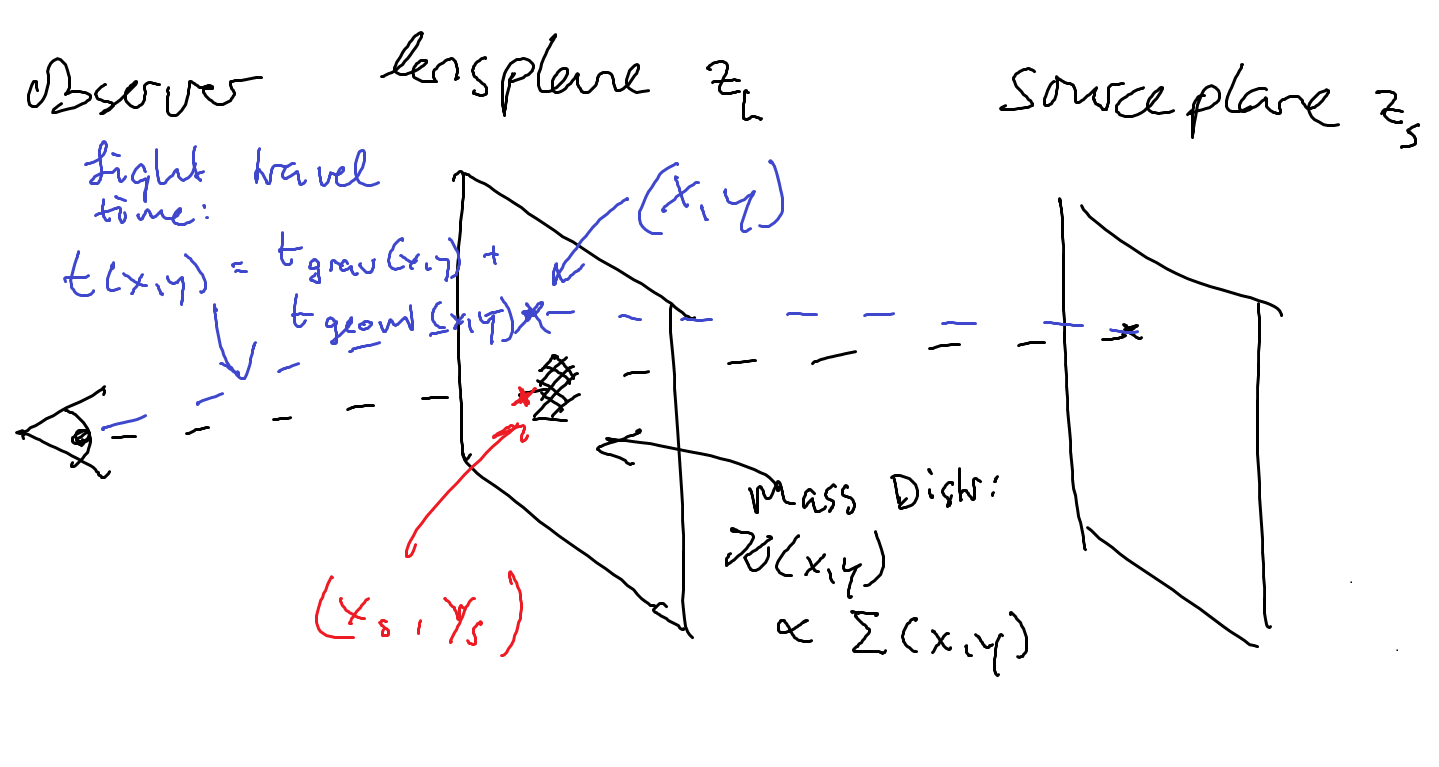
\includegraphics[width=\textwidth]{imgs/sketch_arrtime}
\end{frame}


\begin{frame}
	\frametitle{light travel time}
	\begin{block}{Fermat’s Principle}
		\begin{eqnarray}
			t(x,y) &=& t_\text{geom} + t_\text{grav} \\
			t_\text{geom} &\propto & (x - x_s)^2 + (y-y_s)^2 \\
			t_\text{grav} &=& \left\langle t_\text{grav}(x_\subcirc,y_\subcirc) \right\rangle + (1+z_L) \frac{2G}{c^3} M(x_\subbullet,y_\subbullet)
		\end{eqnarray}
	\end{block}
\end{frame}



%\subsection*{Arrival Time Surface}

\begin{frame}
  \frametitle{Arrival Time Surface}
  \begin{columns}[c]
  	\begin{column}{0.45\textwidth}
	  	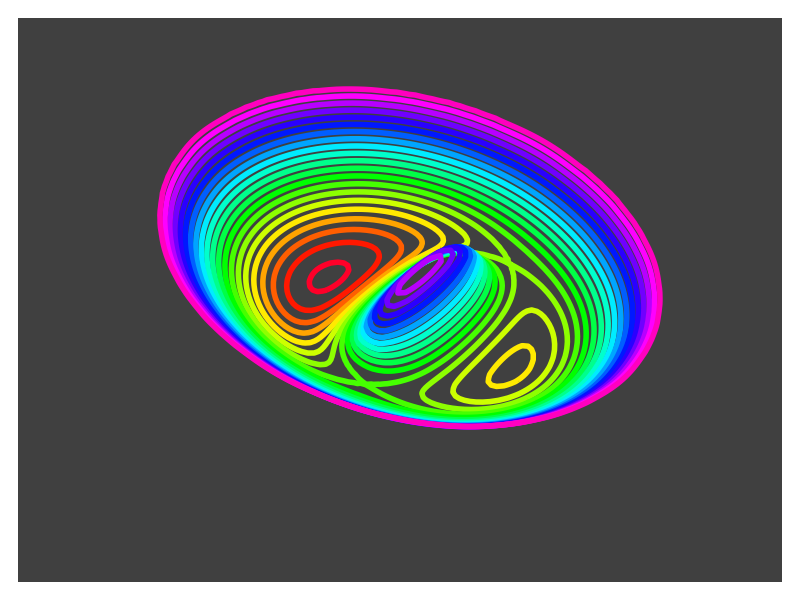
\includegraphics[width=\textwidth]{imgs/arriv_2}
  	\end{column}
  	\begin{column}{0.45\textwidth}
	  	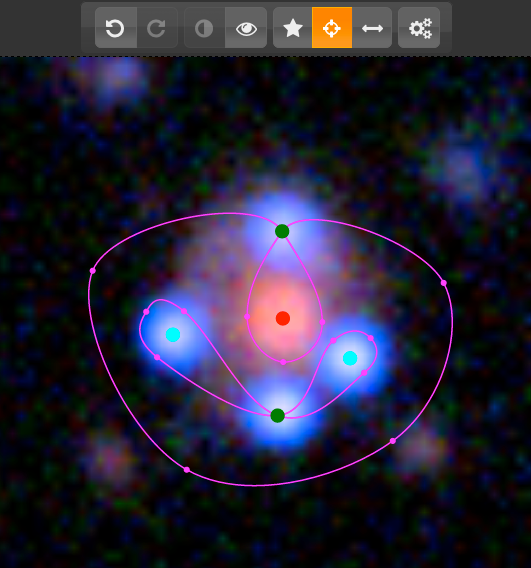
\includegraphics[width=\textwidth]{imgs/screenshot}
  	\end{column}
  \end{columns}
\end{frame}



%\subsection{Demonstration}

 \begin{frame}
   \frametitle{SpaghettiLens}
 
   \begin{columns}[c]
   \begin{column}{0.5\textwidth}
     \begin{itemize}
       \item Extremal Points (Images)
       \item Self Intersecting Contour Lines
     \end{itemize}
     
     \footnotesize{\url{http://labs.spacewarps.org/spaghetti/}}
 
   \end{column}\begin{column}{0.5\textwidth}
     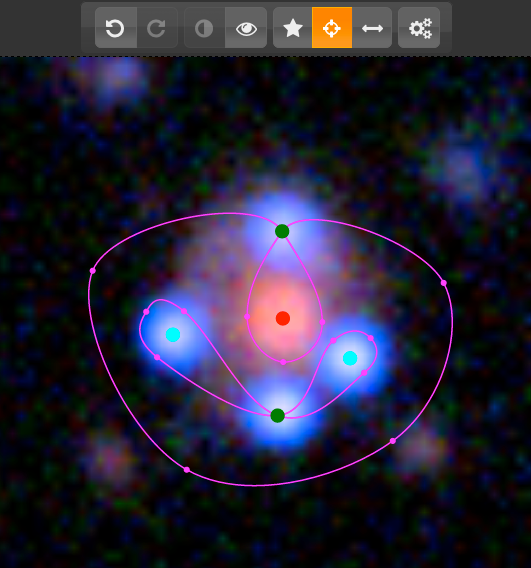
\includegraphics[width=\textwidth]{imgs/screenshot}
   \end{column}
   \end{columns}
 \end{frame}





\section{Results}
%\subsection{SpaceWarps Volunteers}

 \begin{frame}
   \frametitle{SpaceWarps Setup \& Results}
   \begin{itemize}
     \item CFHT Legacy Survey
     \item about 11 million classifications
     \item 29 promising (59 total) new lens candidates
   \end{itemize}
   
   \begin{block}{SpaceWarps: II New Gravitational Lens Candidates...\footnote{arxiv:1504.05587}}
     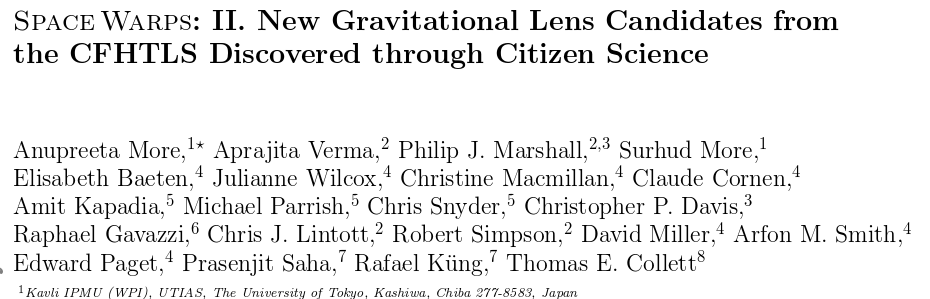
\includegraphics[width=\textwidth]{imgs/paper_sw2}
   \end{block}

 \end{frame}


 \begin{frame}
   \frametitle{SpaghettiLens Results: Tests of Perfomance}
   \begin{itemize}
     \item use simulated lenses
     \item let volunteers model them
     \item recover Einstein Radii
     \item Volunteers perform well!
   \end{itemize}

   \begin{block}{Gravitational Lens Modelling in a Citizen Science Context\footnote{arxiv:1502.00008}}
     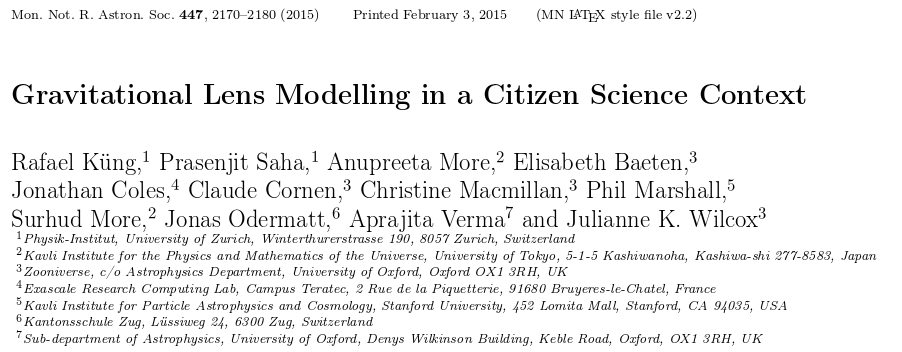
\includegraphics[width=\textwidth]{imgs/paper_sl1}
   \end{block}

 \end{frame}



 \begin{frame}
   \frametitle{SpaghettiLens Results: Stellar vs Lensing Mass}

   \begin{columns}[c]
   \begin{column}{0.5\textwidth}
     \begin{itemize}
       \item lensing mass against the stellar mass of the candidate lens galaxies
       \item stellar mass fraction of order 20 percent
       \item with decreasing trend for the most massive galaxies
       \item expected for early type galaxies
       \item outliers? Maybe non-lenses (not yet spectroscopically confirmed)
     \end{itemize}
 
   \end{column}\begin{column}{0.5\textwidth}
     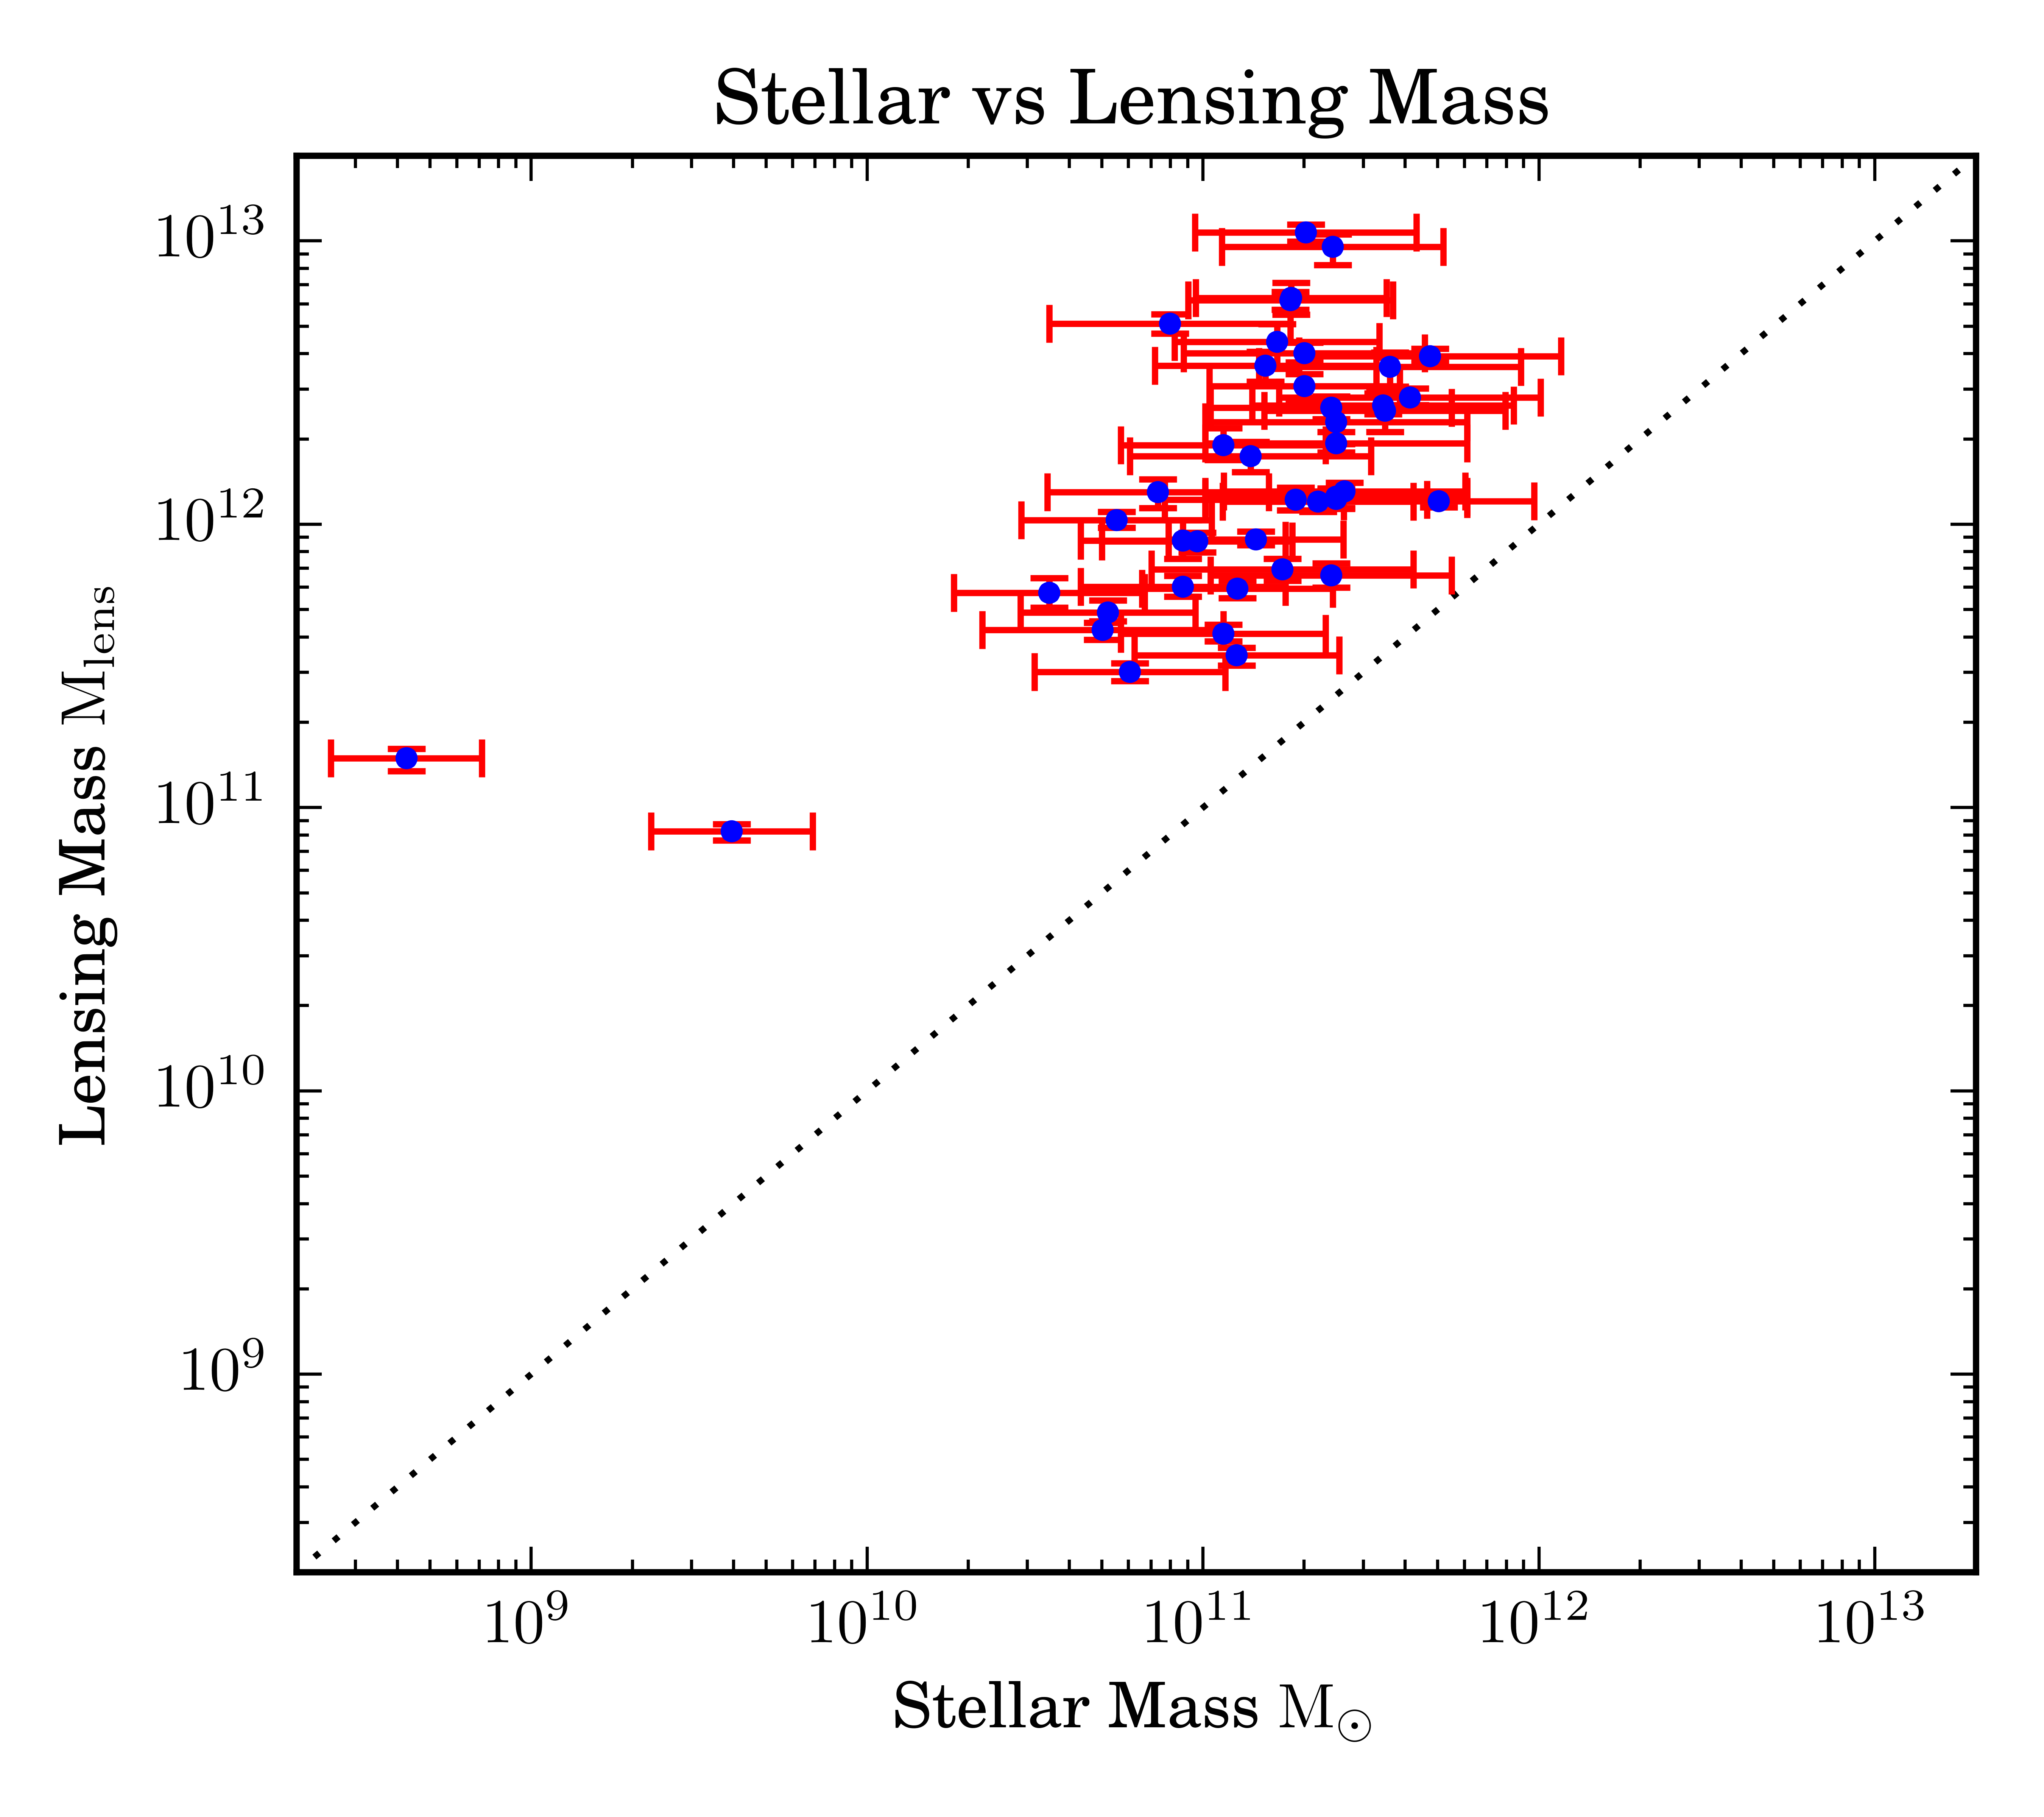
\includegraphics[width=\textwidth]{imgs/plot}
   \end{column}
   \end{columns}

 \end{frame}







%\section*{Conclusions}
%
%\begin{frame}
%  \frametitle{Conclusions}
%  \begin{itemize}
%    \item Volunteers can model lenses
%    \item They do it comparably well to a scientist
%    \item They like doing it
%    \item Collaborative Modelling
%  \end{itemize}
%\end{frame}






\section{Outlook}

\begin{frame}
  \frametitle{Outlook}
  We are currently working on:
  \begin{itemize}
  	\item fit parametrized models to the free-form mass distributions (Lucy Oswald)
    \item determination of photometric red shifts
    \item estimate stellar populations (using galfit, SExtractor)
  \end{itemize}
\end{frame}



\subsection*{Questions?}

\begin{frame}
  \frametitle{Questions?}
  Questions? \\
  rafael.kueng@uzh.ch
\end{frame}




\appendix

\begin{frame}
  \frametitle{Appendix}
\end{frame}

\begin{frame}
  \begin{align}
    A_t &= A_\text{geom} + A_\text{grav}\\
    A_\text{geom} &= \frac{1}{2}\left(x^2+y^2\right)\\
    \nabla^2 A_\text{grav}\left(x,y\right) &= -2\kappa\left(x,y\right)\\
    A           &= \frac{cD_L}{(1+z_L)^2} \frac{D_{LS}}{D_S} \times t \\
    \kappa(x,y) &= \frac{4\pi G}{c^2} \frac{D_L}{1+z_L} \frac{D_{LS}}{D_S} \times \Sigma(x,y)
  \end{align}
  
\end{frame}




\end{document}